\documentclass{ximera}

\input{../preamble.tex}

\title{Explanation and Proof}
\author{Jenny Sheldon}

\begin{document}

\begin{abstract}
We get started with geometry.
\end{abstract}
\maketitle


\section{Activities for this section:} 
\link[Triangle puzzle]{https://ximera.osu.edu/m4t/elementaryActivities/SemesterTwoPacket/elementaryActivities/Preliminaries/TrianglePuzzle}

\section{Explanation and proof}

Geometry has a pretty bad reputation. One of the reasons might be things like this, that you may have seen in high school.

\begin{theorem}
	Prove that if two sides of a triangle are congruent, then the angles opposite those sides are congruent. In other words, given that $\overline{AB} \simeq \overline{AC}$ in the figure below, prove that $\angle B \simeq \angle C$.
	\begin{image}
	\begin{tikzpicture}
		\draw[thick] (0,0)--(2,0)--(1,4)--(0,0);
		\node[left] at (0,0) {$B$};
		\node[above] at (1,4) {$A$};
		\node[right] at (2,0) {$C$};
		\draw[dashed] (1,4)--(1,0);
		\node[below] at (1,0) {$D$};
	\end {tikzpicture}
	\end{image}
\end{theorem}

\begin{proof}

\begin{tabular}{l|l} \hline
{\bf Statement} & {\bf Reasoning} \\ \hline
$\overline{AB} \simeq \overline{AC}$ & Given \\ \hline
Construct a bisector of $\angle A$ & Every angle has a bisector. \\ \hline
$\angle BAD \simeq \angle CAD$ & Definition of angle bisector \\ \hline
$\overline{AD} = \overline{AD}$ & Reflexive property \\ \hline
$\triangle ABD \simeq \triangle ACD$ & SAS Postulate \\ \hline
$\angle B \simeq \angle C$ & CPCTC \\ \hline
\end{tabular}
\end{proof}

Don't worry: we're not planning to make this kind of proof in this class unless you want to. And we don't expect you to be able to decode everything in the proof above right now. 

But perhaps you can see my point about geometry's bad reputation. The example above is actually a very nice example of a particular class of proofs, but this version is hard to understand.  Besides the alphabet soup of letters that makes this tough to decipher, why would we even make one of these in the first place? And once we've made one of them, why continue making them for a whole host of other statements? What even is a proof, anyway, and why would anyone want one? 

I'm glad you asked!

\section{Proof in Mathematics}

A mathematical proof is an argument about the truth of a particular statement. The statement itself is often called a theorem or a proposition. Sometimes mathematicians even get fancy and call them ``lemmas''. All of these words are synonyms for the same thing: a statement that's true. And once we make a statement and claim that it's true, we have to convince people that it's actually true, which is where the idea of a proof comes in. 

This should hopefully feel a little familiar, even if the terminology is strange. For instance, you might make a statement like, ``My best friend is the most amazing person on Earth'' and someone else might reasonably ask you to explain why that statement is true. Your explanation would probably include details about who your best friend is and what kind of amazing things you have seen them do. Since your statement is pretty broad (the most amazing person on Earth is a pretty high bar!) you would likely need lots of examples to really convince someone else. Or perhaps you have already met every person on Earth, somehow, and you could compare your best friend to each of them. Your statement is a theorem, and your argument for why the statement is true is like a proof.

Turning to an example you might have seen before in a math class, let's look at the following.
\begin{example}
We could make a statement like ``the sum of two odd numbers is an even number''. Since this is a statement about any two odd numbers, we can't really just try some examples to see whether not this statement is true. We need a more general argument. We might start by saying that an even number is a number that's divisible by $\answer[given]{2}$ with no remainder, and an odd number is a number that's divisible by $2$ with a remainder of $\answer[given]{1}$.  If we apply these definitions to this particular case, we start with two different odd numbers. Each of them can be arranged into groups of $2$ with one remainder. We can draw an example of adding two odd numbers together. We will have a collection of dots organized into groups of $2$ with one leftover, and another collection of dots organized into groups of $2$ with one left over. These two numbers don't have to be the same size, and we will use some dots in the middle of the groups of two to indicate that there could be any number of these groups.
\begin{image}
\begin{tikzpicture}
\foreach \x in {0, 1, 2, 4, 5, 6} \foreach \y in {0, 1} \draw[fill=pink] (\x, \y) circle (3pt);
\foreach \x in {10, 12} \foreach \y in {0, 1} \draw[fill=violet] (\x, \y) circle (3pt);
\draw[fill=pink] (7,0) circle (3pt);
\draw[fill=violet] (9,1) circle (3pt);
\node at (8, 0.5) {$+$};
\node at (3, 0.5) {$\dots$};
\node at (11, 0.5) {$\dots$};
\end{tikzpicture}
\end{image}
If we combine together the leftover objects into another group of $2$, we have made groups of $2$ with $\answer[given]{0}$ leftovers, meaning the sum of these two numbers is even because it satisfies our definition of an even number. We'll show circles around the original groups of two, and another circle around the two extra objects making another group of $2$.
\begin{image}
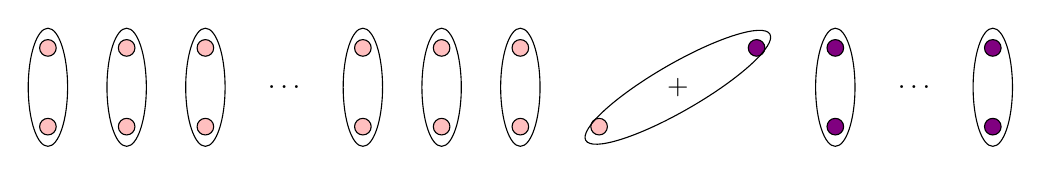
\begin{tikzpicture}
\foreach \x in {0, 1, 2, 4, 5, 6} \foreach \y in {0, 1} \draw[fill=pink] (\x, \y) circle (3pt);
\foreach \x in {10, 12} \foreach \y in {0, 1} \draw[fill=violet] (\x, \y) circle (3pt);
\draw[fill=pink] (7,0) circle (3pt);
\draw[fill=violet] (9,1) circle (3pt);
\node at (8, 0.5) {$+$};
\node at (3, 0.5) {$\dots$};
\node at (11, 0.5) {$\dots$};
\foreach \x in {0, 1, 2, 4, 5, 6, 10, 12} \draw (\x, 0.5) ellipse (0.25cm and 0.75cm);
\begin{scope}[shift={(8, 0.5)}]
\draw[rotate=120] (0,0) ellipse (0.3cm and 1.35cm);
\end{scope}
\end{tikzpicture}
\end{image}

The statement is a theorem, and our argument is its proof. If you felt like it, you could even organize this proof into two columns like the one above.
\end{example}

The previous proof was pretty simple, but I hope you can now imagine many more complicated theorems that you have already stated in your mathematics education, and perhaps you've even proven some of them. The two-column proof above is a way of organizing a proof whose goal is to remind you that while you are making your proof, you need to give a justification for every step you take. In other words, after every sentence you write, you should ask yourself ``why?'' and then be sure that the ``why'' is included in your proof.

\emph{Proof is at the heart of mathematics.} Writing a proof is a bit like conducting an experiment in science: you have a hypothesis, and then you want to test out that hypothesis to see if it will hold. A theorem is a little like a hypothesis, and a proof is a little like a successful experiment (though there are some important differences as well). Writing a proof is a bit like writing a paper in English: you start with a point that you'd like to make, which is like a theorem. Then, the paper itself gives all the arguments for why that point is valid, which is like a proof. A proof could be like a beautiful musical composition: the theorem would be the emotions that the composer wants the audience to feel, and the composition itself takes the audience through those emotions.

 \emph{Proof allows mathematics to be dependable.} A good proof is valid as long as all of the assumptions in the argument hold. Proof isn't about opinion, and doesn't change as time goes by. Once a theorem has been proven, it remains proven for the rest of history. For this reason, a proof has to be carefully constructed without holes in the logical reasoning or jumps in the line of thinking. Especially in geometry, we have to be careful not to consider only a few examples but instead consider all examples that could ever be made. This is tricky -- and a bit like trying to convince someone that your best friend is the most amazing person on Earth! Thankfully, mathematics has definitions that help us to truly consider all shapes of a certain type, not just a few examples.
 
\emph{Proof allows mathematics to build on itself.} Once a theorem is known without a doubt, we can use it to prove other theorems and to build more mathematics. Mathematicians are still extending the reach of mathematical knowledge today, building off of what past mathematicians have proven.
 
 Finally, \emph{proof can be beautiful}. Proof shows us how the world works. We can find connections in places we never expected. We can be surprised by how changing tiny details can make a big difference in an outcome. We can be delighted in the certainty of knowing things. We can refine our proofs over time to make the main ideas more clear and concise. We can be proud of our accomplishments when we finish a tough argument.  I hope that you will catch at least a glimpse of the beauty of proof in this course!


\section{Proof in this class}

Hopefully, you have already picked up that we are going to ask you to prove things in this course. But hopefully you have also picked up that this isn't really different than what we asked you in the previous course. The explanations you learned to write in that course are proofs, and so we will continue to write proofs in this course. Of course, if this doesn't sound at all familiar, you're still welcome here and we'll have plenty of conversations about what we expect in an explanation. We are happy to support you no matter what prior knowledge you're bringing to the course.

No matter where you took the first semester of this course, take a few moments to review the section on \link[Explanations]{https://ximera.osu.edu/m4t/elementaryTeachersOne/elementaryReading/Numbers/Explanations} that we considered in our first course. Finally, remember that a good explanation usually contains at least the following.

\begin{itemize}
	\item A definition for the relevant item(s) in the problem.
	\item An explanation of how the definition(s) apply to the particular case you are working on.
	\item A picture or sequence of pictures.
	\item An explanation for how you want the reader to be looking at your picture, or why you drew this particular picture at this particular point in time.
\end{itemize}

We are here for you, and happy to talk about your explanations and proofs at any point in time.


\end{document}
